\documentclass[12pt]{article}
\usepackage[margin=1in]{geometry} 
\usepackage{amsmath}
\usepackage{tcolorbox}
\usepackage{amssymb}
\usepackage{amsthm}
\usepackage{lastpage}
\usepackage{fancyhdr}
\usepackage{accents}
\usepackage{mathtools}
\usepackage{tikz}
\usepackage{gensymb}
\usepackage{listings}
\usepackage{graphicx}
\usepackage{circuitikz}
\usepackage{pgfplots}
\pagestyle{fancy}
\setlength{\headheight}{40pt}

\lstset{
  basicstyle=\ttfamily,
  columns=fullflexible,
  frame=single,
  breaklines=true,
  postbreak=\mbox{\textcolor{red}{$\hookrightarrow$}\space},
}

\newenvironment{solution}
  {\renewcommand\qedsymbol{$\blacksquare$}
  \begin{proof}[Solution]}
  {\end{proof}}
\renewcommand\qedsymbol{$\blacksquare$}

\newcommand{\ubar}[1]{\underaccent{\bar}{#1}}

\usetikzlibrary{calc,patterns,angles,quotes}
\usepackage{amsmath}

\title{Quantitative Engineering Analysis \\ Gauntlet Challenge: Navigating the Gauntlet (Level 3)}

\author{Rohil Agarwal, Wesley Soo-Hoo \\ Olin College of Engineering \\ ENGX2001 Spring 2020}
\date{\today}

\begin{document}
\begin{titlepage}
\maketitle

\begin{center}
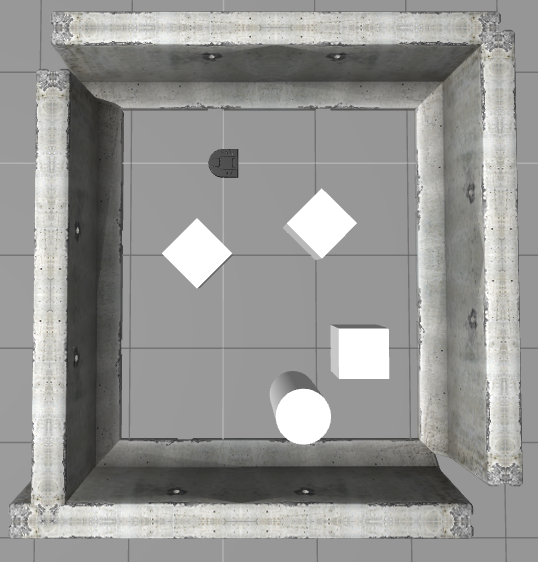
\includegraphics[width=.75\textwidth]{img/CaptureGauntletCover.PNG}
\end{center}
\end{titlepage}

\section{Introduction}
In this document, we present our journey to attempt to complete the infamous  Gauntlet Challenge. In this challenge, our Neato navigates the treacherous Gauntlet, which is made up of four imposing walls, within which lie multiple menacing obstacles and the metaphorical Holy Grail, the object which represents the Neato’s sole purpose of existence: the wondrous Barrel of Benevolence (BoB).

The journey was not going to be easy for our Neato. We decided to conquer Level 3, the most challenging challenge of all possible challenges. For this level of the challenge, we scanned the Gauntlet at the beginning using LIDAR, identified and fit the BoB, the obstacles, and the walls using RANSAC, and placed sources and sinks based on this to create a potential field of the gauntlet. We then used gradient descent to traverse the pre-planned path.

There were a couple obstacles we ran into (pun intended) during this challenge. One issue was that when we tried using RANSAC for the circle rather than the lines, since some of the square obstacles had more points detected by the LIDAR, the algorithm tried to fit the square obstacles with circles. We realized that if you get a good circle fit, there won't be any points close to the circle that aren't inliers, but with the square obstacles there will be. Therefore, we created a new category of "near matches,” or points that are almost inliers but not quite, and said that the optimal circle fit occurred when there were none of these near matches.

The Neato traversed a predetermined path that was generated based on the gradient of the potential field given by an equation that mathematically describes the Gauntlet features as sources and sinks. The equation of the potential field, which was based on the intial LIDAR scan, was given by the function

\begin{align*}
    \boldsymbol{f}(x,y) = -&\boldsymbol{w_1}(\ln{\sqrt{(x-x_c)^2+(y-y_c)^2}})\,+ \\
    &\boldsymbol{w_2}(\ln{\sqrt{(x-x_{wp})^2+(y-y_{wp})^2}})\,+ \\
    &\boldsymbol{w_3}(\ln{\sqrt{(x-x_{op})^2+(y-y_{op})^2}})
\end{align*}

\vspace{.1in}

Where:

\begin{itemize}
    \item $w_1$, $w_2$, $w_3$ are the weights for the BoB, wall points, and obstacle points
    \item $x_c$, $y_c$ are the coordinates of the center of the BoB's 
    \item $x_{wp}$, $y_{wp}$ are the coordinates of the points that make up the walls
    \item $x_{op}$, $y_{op}$ are the coordinates of the points that make up the obstacles 
\end{itemize}

In reality, the equation we used included additional versions of the second and third addends for each of the points in the wall and obstacles, respectively. This was because, unlike the BoB the walls and obstacles did not have center points that could be used to sum up the potential field created by the feature. The weights allowed us to adjust the impact of these addends accordingly (BoB addend was given a much larger weight than the addends for each of the points that made up the walls and obstacles). We used for loops to add these additional addends to the function.

\section{Experimental Validation}

The Neato moved 2.32 meters over a period of 27 seconds to get to the BoB. These numbers were collected using the \textit{collectDataset$\_$sim.m} script provided to us. The time was pulled directly from the dataset, while the distance was calculated by using the wheel positions and time to get the wheel velocities, using this to get the linear speed, and then multiplying this by time to get the distance traveled.

See the theoretical and experimental paths in \textbf{Figure \ref{fig:bothpaths}}, at the bottom of this document.

\begin{figure}[h]
    \centering
    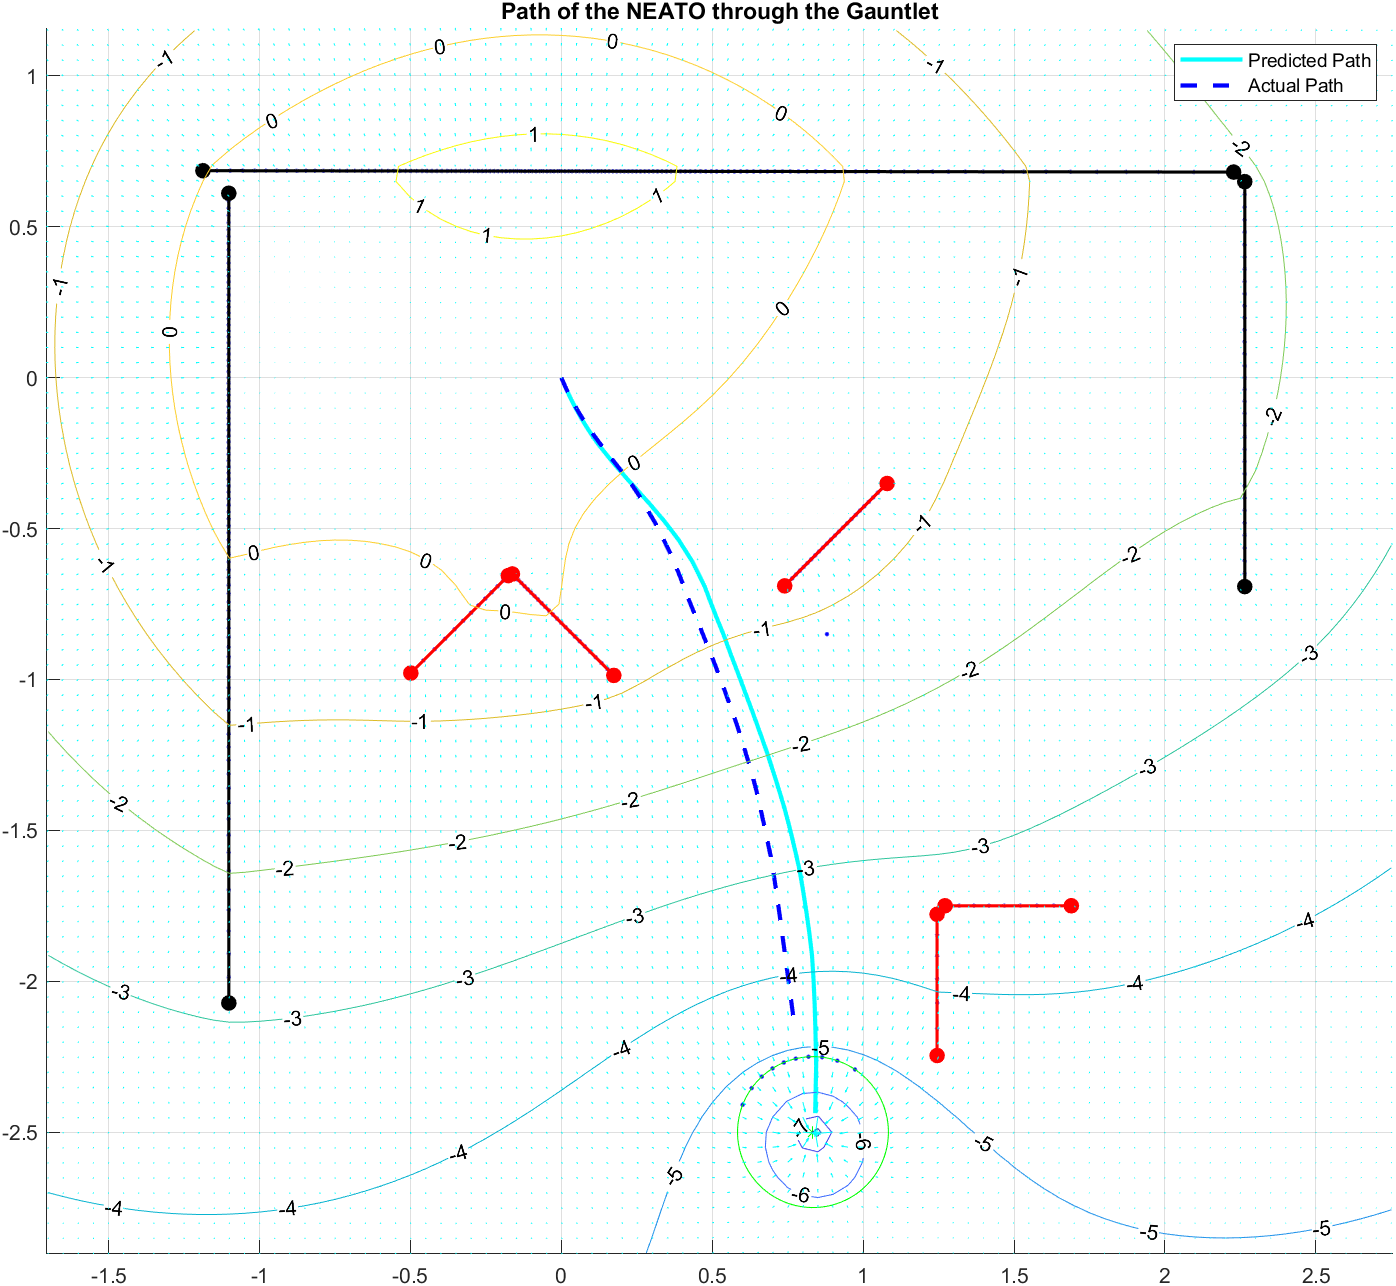
\includegraphics[width=0.65\textwidth]{img/paths.png}
    \caption{A map of the Gauntlet overlaid with the intended path of gradient descent and the actual path the Neato took (calculated from the wheel encoder data).}
    \label{fig:bothpaths}
\end{figure}

\section{Video}
The video of the Neato making its perilous journey to the Barrel of Benevolence can be found here:
\url{https://youtu.be/NlUoVpO0FB0}

\section{Complete Code}
The code can be found here: \url{https://github.com/wsh32/qea/tree/master/pset19}


\end{document}